\newpage
\section{Aufgabe 1}
\subsection{Aufgabenstellung}
\begin{itemize}
	\item Installieren und konfigurieren Sie die Entwicklungsumgebung Energia für das Tiva C Series LaunchPad gemä\ss{} der beigelegten Anleitung oder Anweisungen auf der Energia-Webseite.
	\item Schlie\ss{}en Sie das Launchpad an und wählen Sie in der Entwicklungsumgebung die entsprechende Plattform (Tools -> Board -> $"$Launch Pad (Tiva C) w/ TM4C123 (80MHz)$"$) aus. Ggf. müssen Sie das Board über den Boardverwalter installieren (Tools -> Board -> Boards Manager).
	\item Wählen Sie aus dem Menü der Entwicklungsumgebung das Programm $"$Blink$"$ (findet sich unter File -> Examples -> 1. Basics) aus.
	\item Ändern Sie in dem Programm das Zeitintervall von 1s auf 4s. Vermeiden Sie $"$magic numbers$"$.
	\item Schalten Sie unter $"$File -> Preferences$"$ den $"$verbose output$"$ für $"$compilation$"$ und $"$upload$"$ ein.
	\item Prüfen Sie Ihr Programm mittels der Entwicklungsumgebung ($"$Verify code after upload$"$).
	\item Laden Sie das geänderte Programm auf das Board hoch (Pfeilsymbol $"$Upload$"$).
\end{itemize}
\subsection{Durchführung}
Zunächst wurde die Entwicklungsumgebung \textit{Energia} für das \textit{Tiva C Series LaunchPad} nach der gegebenen Anleitung, auf einem Windows 10 PC, installiert.

\begin{figure}[h]
	\centering
	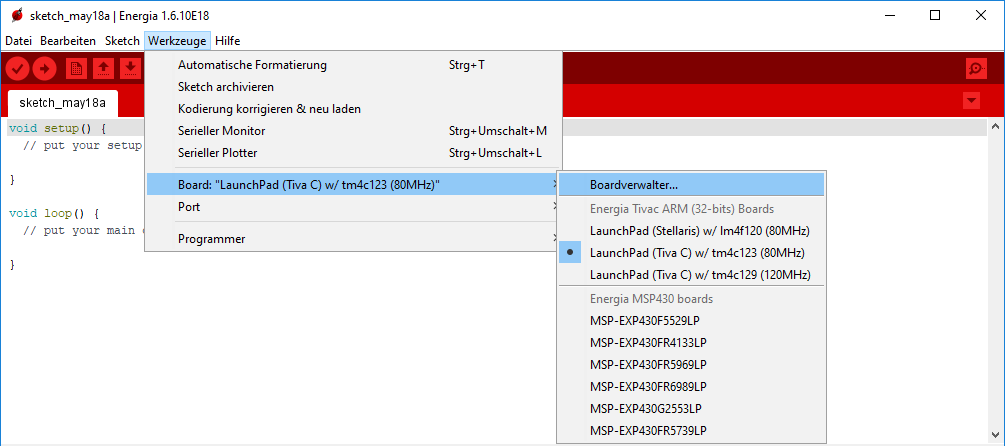
\includegraphics[width=0.7\linewidth]{images/addTM4C123}
	\caption{Öffnen des Board Manager}
	\label{fig:addTM4C123}
\end{figure}
\noindent Wie oben in Abbildung 1 gezeigt wurde der Board Manager gestartet und durch ihn dann das \textit{TM4C123} installiert.
\newpage
\begin{figure}[h]
	\centering
	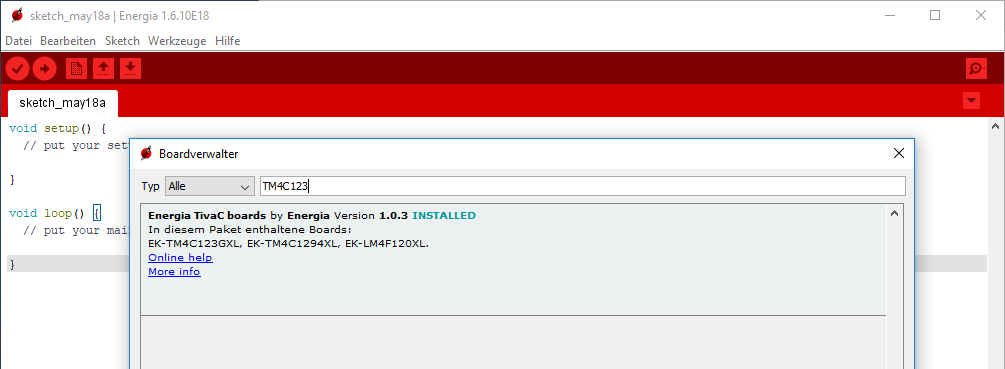
\includegraphics[width=0.7\linewidth]{images/addTM4C123(2)}
	\caption{Suchen des TM4C123}
	\label{fig:addTM4C123(2)}
\end{figure}
\noindent Wie in Abbildung 1 zu sehen ist das \textit{LaunchPad (Tiva C) w/ tm4c123 (80MHz)} bereits ausgewählt.\\ \\
Als nächstes wurde das Beispiel \textit{Blink} überarbeitet und das Zeitintervall des Blink-Programms von 1s auf 4s gesetzt. Dazu wurde die Variable $BLINK\_INTERVALL$ erstellt um \textit{magic numbers} zu vermeiden. $BLINK\_INTERVALL$ wurde mit dem Wert 4000 definiert und an den den Befehl \textit{delay} übergeben.
\begin{lstlisting}[label=lst:bash]
/*
  Blink
  The basic Energia example.
  Turns on an LED on for one second, then off for one second, repeatedly.
  Change the LED define to blink other LEDs.
  
  Hardware Required:
  * LaunchPad with an LED
  
  This example code is in the public domain.
*/

// most launchpads have a red LED
#define LED RED_LED
#define BLINK_INTERVALL 4000

//see pins_energia.h for more LED definitions
//#define LED GREEN_LED
  
// the setup routine runs once when you press reset:
void setup() {                
  // initialize the digital pin as an output.
  pinMode(LED, OUTPUT);     
}

// the loop routine runs over and over again forever:
void loop() {
  digitalWrite(LED, HIGH);   // turn the LED on (HIGH is the voltage level)
  delay(BLINK_INTERVALL);    // wait for 4 seconds
  digitalWrite(LED, LOW);    // turn the LED off by making the voltage LOW
  delay(BLINK_INTERVALL);    // wait for 4 seconds
}
\end{lstlisting}
\noindent \\Zuletzt wurden die Einstellungen anhand der Aufgabenstellung, wie in Abbildung 3, angepasst, das Programm mit der Entwicklungsumgebung geprüft und auf das Board geladen.
\begin{figure}[h]
	\centering
	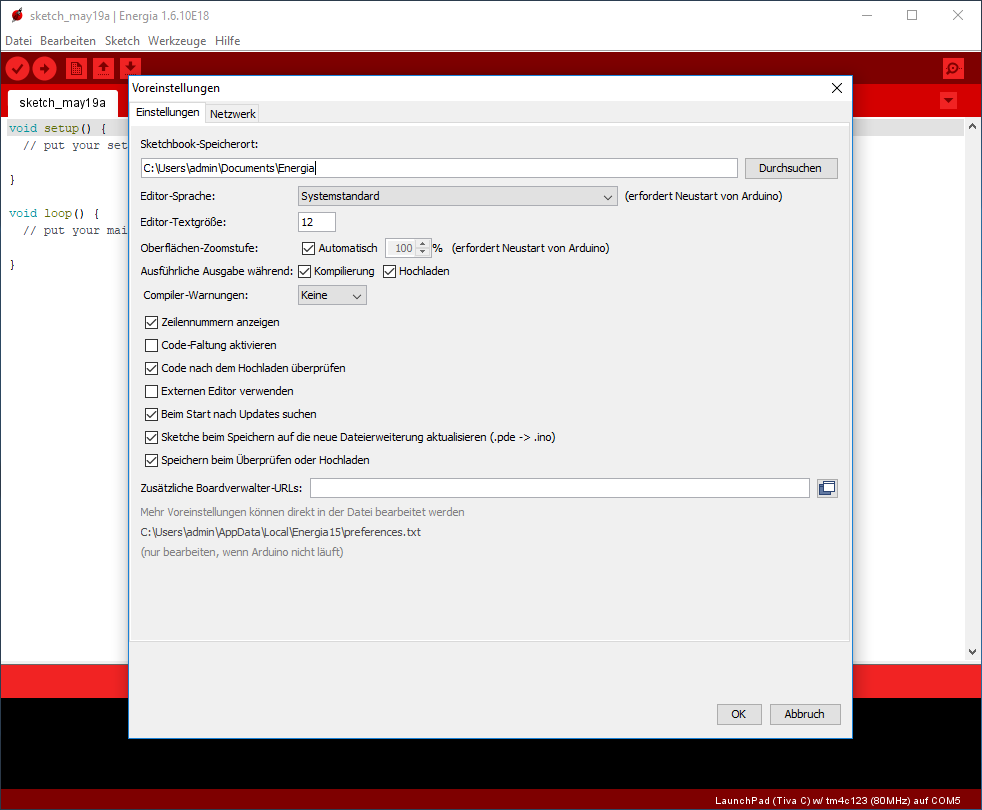
\includegraphics[width=0.7\linewidth]{images/Settings}
	\caption{Einstellungen}
\end{figure}
\newpage
\section{Aufgabe 2}
Welche generellen Schritte führt die hinter der Energia-Entwicklungsumgebung liegende Toolchain aus (Tipp: Betrachten Sie dafür den $"$verbose output$"$)?\\ \\
Zuerst werden die  .cpp und .c zu .cpp.o und c.o Dateien compiliert. Dann werden die einzelnen .cpp.o und .c.o zu einer core.a Datei compiliert. Danach werden die Libs zusammen gelingt.
Und auf das Board geflasht.\\ \\
Aus welchen Tools besteht die Toolchain (der letzte Schritt ist das Hochladen auf das Board)?\\ \\
Die Toolchain besteht aus folgenden Tools:
\begin{itemize}
\item arm-none-eabi-g++     : Compiliert .cpp Dateien.
\item arm-none-eabi-gcc     : Compiliert .c Dateien.
\item arm-none-eabi-ar      : Compiliert .cpp.o und .c.o Dateien zu einer core.a Datei
\item arm-none-eabi-objcopy : Generiert die Binär-Datei.
\item dslite                : Flasht die Binär-Datei auf das Board.
\end{itemize}
\section{Aufgabe 3}
Lokalisieren Sie in den Verzeichnissen der Energia-Installation das Linker-Skript $"$Im4fcpp\_blizzard$"$ (Tipp: Schauen Sie Sich den Linker-Schritt in der Konsole an).\\ \\
C:\textbackslash Users\textbackslash admin\textbackslash AppData\textbackslash Local\textbackslash Energia15\textbackslash packages\textbackslash energia\textbackslash hardware\textbackslash  tivac\textbackslash 1.0.3\textbackslash variants\textbackslash EK-TM4C123GXL\textbackslash lm4fcpp\_blizzard.ld\\ \\
Welche Aufgaben erfüllt ein Linker-Skript?\\ \\
Ein Linker-Skript konfiguriert die Einstellungen für ein Energia C++ Programm\\ \\
Was beschreiben die einzelnen Zeilen in dem Block \textit{Memory}?\\ \\
In dem Block wird die Startadresse, die Speichergro\ss{}e und die Lese-Schreib-Rechte für den Flash-Speicher und den RAM definiert. Der Flash-Speicher darf Lesen und Ausführen, beginnt bei der Adresse 0x00000000 und endet bei der Adresse 0x00040000 und die Speichergro\ss{}e beträgt 256kB. Der RAM darf Lesen, Schreiben und Ausführen, beginnt bei der Adresse 0x20000000 und endet bei der Adresse 0x20008000 und die Speichergro\ss{}e beträgt 32kB.
\newpage
\section{Aufgabe 4}
\begin{figure}[h]
	\centering
	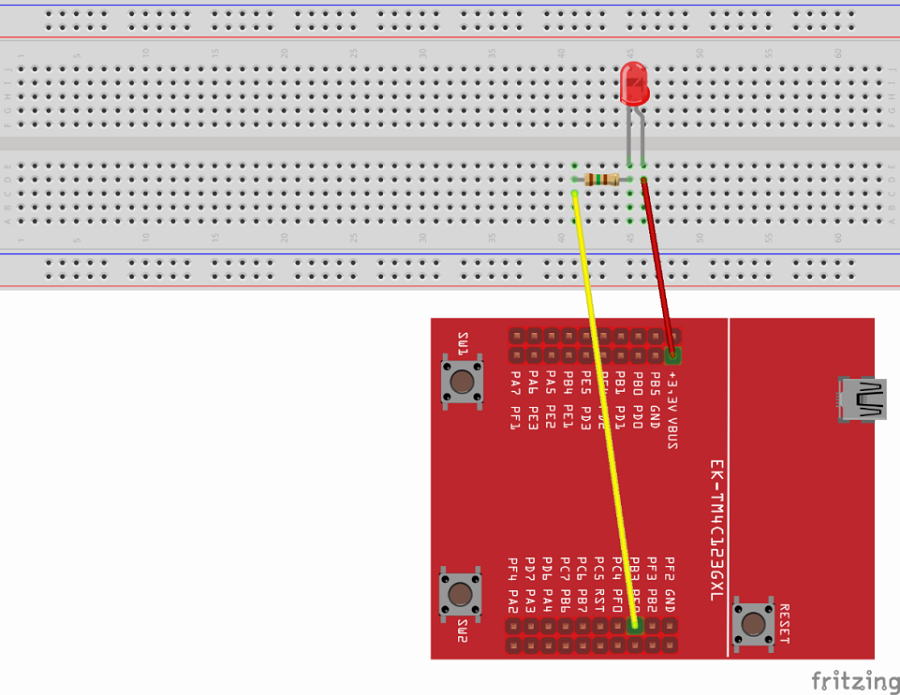
\includegraphics[width=0.7\linewidth]{images/sosSchaltung}
\end{figure}
\noindent Schreiben Sie ein Programm, das mittels einer LED ein SOS signalisiert. Bauen Sie dafür die abgebildete Schaltung auf (150$\Omega$ Widerstand, LED wird angeschlossen an den Pin PB\_3) oder verwenden Sie wie oben die Onboard-LED. Strukturieren Sie Ihr Programm dabei \textit{sinnvoll} zur Wiederverwendung mittels Verwendung von Funktionen.\\ \\
Als erstes wurde der Angesprochene Pin $PB\_3$ und die Geschwindigkeiten $SPEED\_S$ und $SPEED\_O$ definiert. In der Funkton \textit{setup} wird das Ansprechen des Pins vorbereitet. Der Funktion \textit{character} muss ein Integer übergeben werden, dieser bestimmt wie lange die LED an bleibt. Zum Schluss wird in der Funktion \textit{loop} in for-Schleifen die Funktion \textit{character} aufgerufen um S.O.S zu blinken.
\begin{lstlisting}[label=lst:bash]
#define PIN PB_3
#define SPEED_S 500
#define SPEED_O 2000

void setup() {
  // put your setup code here, to run once:
  pinMode(PIN, OUTPUT); 
}

void character(int speed) {
  digitalWrite(PIN, LOW);
  delay(speed);
  digitalWrite(PIN, HIGH);
  delay(speed);
}

void loop() {
  for (int x = 1; x <= 3; x++) {
    character(SPEED_S);
  }
  for (int x = 1; x <= 3; x++) {
    character(SPEED_O);
  }
  for (int x = 1; x <= 3; x++) {
    character(SPEED_S);
  }
  delay(2000);
}
\end{lstlisting}
\section{Aufgabe 5}
Lokalisieren Sie in der Energia-Umgebung die folgenden Dateien:
\begin{itemize}
	\item Energia.h
	\item main.cpp
\end{itemize}
und vollziehen Sie die Funktionsweise des Programmablaufs (s. main.cpp) nach.\\ \\
Die Energia.h und die main.cpp Datei befinden sich in folgenden Ordner\\
C:\textbackslash Program Files\textbackslash energia-1.6.10E18\textbackslash hardware\textbackslash energia\textbackslash msp430\textbackslash cores\textbackslash msp430\\
In \textit{Energia.h} befinden sich nur Definitionen (z. B. HIGH und LOW). Dort finden sich auch Definitionen von Funktionen wie \textit{delay} und \textit{sleep}. In der \textit{main.cpp} wird die \textit{Energia.h} Datei inkludiert und die \textit{main} Funktion definiert. In der \textit{main} Funktion wird zuerst die init() Funktion aufgerufen. Dann die vom Programmierer erstellte \textit{setup()} Funktion aufgerufen, so wie die \textit{loop()} Funktion, welche sich in einer Endlosschleife befindet.\\ \\
Warum reicht es aus, nur die Funktionen \textit{setup} und \textit{loop} für ein Energia-Programm (Sketch) zu implementieren?\\ \\
Durch die Beschreibung der \textit{main} Funktion wird auch klar wieso es reicht wenn man nur \textit{setup} und \textit{loop} implementiert. Diese beiden Funktionen werden in der \textit{main} Funktion aufgerufen.
